\documentclass[a4paper,10pt]{article}
%\usepackage[utf8x]{inputenc}
\usepackage[utf8]{inputenc}
\usepackage{graphicx}

%opening
\title{Detección automática de malos hábitos de programación con Scratch}
\author{Gregorio Robles, Jesús Moreno}

\begin{document}

\maketitle

\begin{abstract}
Este artículo describe un método de detección automática de dos malos hábitos de programación muy presentes en estudiantes que aprenden a programar con Scratch, como son la repetición de código y el nombrado de objetos, y plantea ideas para tratar de
evitar este tipo de situaciones.

\end{abstract}

\section{Introduction}
Scratch \cite{resnick2009scratch} es un entorno de programación que incluye un lenguaje de programación visual pensado para niños desde 6 años de edad, un entorno de desarrollo y un sitio web donde la comunidad puede alojar sus proyectos, ejecutar, estudiar y reutilizar otros programas, y compartir ideas o sugerencias. Aunque existen otros lenguajes de programación visuales similares, Scratch es sin duda el que más éxito ha tenido y el que se está usando de forma más habitual en todo el mundo, con más de tres millones de usuarios registrados en su web y más de cinco millones de proyectos compartidos en su repositorio \footnote{http://scratch.mit.edu/statistics/}.
\paragraph{}Scratch está siendo utilizado tanto en actividades extraescolares \cite{maloney2008programming, kafai2010entering} o campamentos de verano \cite{adams2010scratching, franklin2013assessment}, como en escuelas \cite{wilson2012evaluation}, institutos \cite{meerbaum2013learning} e incluso universidades \cite{wolz2009starting, malan2007scratch} de todo el mundo, y se ha documentado su capacidad no solo para acercar la programación y la informática a niños y jóvenes con el objetivo de que en el futuro se planteen continuar sus estudios en esta disciplina, sino también su éxito para enseñar conceptos de programación tanto básicos como avanzados.
\paragraph{}Sin embargo, también es posible encontrar trabajos que han detectado ciertos malos hábitos de programación en los estudiantes que aprenden a programar en este entorno \cite{meerbaum2011habits}. En esta línea, en nuestro trabajo como docentes hemos detectado otros malos hábitos o manías que, a pesar de insistir en ellas para tratar de evitarlas, vemos cómo se repiten constantemente en los alumonos que aprenden a programar en este entorno. Como estos hábitos son contrarios a las recomendaciones básicas de la programación, nuestro estudio trata de detectar si son comunes también en los proyectos compartidos en el repositorio y plantear ideas para tratar de evitar este tipo de situaciones.
\paragraph{}En la sección 2 se realiza un repaso sobre Scratch y se revisan trabajos que estudian los aprendizajes demostrados por estudiantes que aprenden a programar en este entorno, así como estudios que automatizan la evaluación automática de estos aprendizajes. En la sección 3 se describe la metodología seguida en nuestro trabajo. La sección 4 recoge los resultados obtenidos. Finalmente, en la sección 5  se explican las conclusiones de nuestro estudio y se ofrecen algunas ideas y sugerencias para futuros trabajos.

\section{Background}

\paragraph{}Scratch es un entorno de programación visual desarrollado por el grupo Lifelong Kindergarten del Media Laboratory del MIT que permite programar proyectos interactivos utilizando un enfoque drag-and-drop con diferentes piezas o bloques tipo \textit{Lego} \cite{resnick2009scratch}. Scratch se diseñó con el objetivo principal de animar a los jóvenes a programar, y la mayoría de sus usarios son aprendices noveles que no tienen experiencia previa en programación \cite{maloney2010scratch}. El entorno está diseñado para animar a los usuarios a que manipulen y modifiquen distintos tipos de elementos multimedia, de forma que niños y jóvenes pueden programar proyectos que les resultan interesantes y atractivos, como historias animadas, juegos y presentaciones interactivas \cite{maloney2008programming}
\paragraph{}Scratch también ofrece un sitio web en el que se publican los proyectos programados por los usuarios, se puede estudiar el código de cada programa, realizar comentarios y sugerencias y reutilizar el código de cualquier proyecto, por lo que cualquiera que quiera comenzar a programar tiene a su disposición una gran cantidad de recursos. Este enfoque, además, ofrece la oportunidad de aprender ciertas habilidades sociales relacionadas con la programación, como compartir y contribuir a la comunidad \cite{scaffidi2012skill}.
\paragraph{}Tal como se mencionaba en la introducción, es posible encontrar muchos trabajos \cite{maloney2008programming, franklin2013assessment,scaffidi2012skill,malan2007scratch} que demuestran que Scratch funciona como herramienta para aprender a programar, ya que existen casos de éxito en distintos nieveles educativos, entornos y disciplinas que muestran que los estudiantes aprenden conceptos como la interacción de usuario, sentencias condicionales, comunicación y sincronización, expresiones lógicas o representación de la información con variables.
\paragraph{}A pesar de estos buenos resultados, Meerbaum-Salant, Armoni y Ben-Ari \cite{meerbaum2011habits} ponen de manifiesto que los estudiantes que aprenden a programar en este entorno demuestran algunos malos hábitos que son contrarios a las buenas prácticas recomendadas. En concreto, demuestran una tendencia excesiva descomposición y un proceso de desarrollo totalmente de abajo a arriba que comienza con bloques individuales de Scratch.
\paragraph{}Con la idea de simplificar el proceso de evaluación del CT ayudando al evaluador con una herramienta de automatización de parte del proceso se creó Hairball \cite{boe2013hairball}, que es un analizador estático de proyectos Scratch inspirado en Lint\footnote{http://www.unix.com/man-page/FreeBSD/1/lint} que trata de detectar posibles errores de programación en un proyecto Scratch, como no inicializar el valor de una variable o el estado de un personaje, enviar mensajes que no son recibidos por ningún programa o incluir código que no llega a ejecutarse.

\section{Methodology}

\paragraph{}En nuestro trabajo como docentes con estudiantes de secundaria, hemos detectado que muchos estudiantes presentan dos malos hábitos de manera recurrente, a pesar de nuestra constante insistencia para tratar de evitarlos, que tienen que ver con el nombrado de objetos y con la repetición de código.

\paragraph{}Por una parte, es muy habitual comprobar que los estudiantes no cambian el nombre de los personajes, que el entorno bautiza como \textit{SpriteX}, donde X es un número incremental, de manera que al crecer el número de personajes de un proyecto resulta complicado saber a qué objeto se refiere una determinada sentencia, contribuyendo así a una mala legibilidad del código, ralentizando la programación del proyecto y complicando su depuración ante posibles errores.
\paragraph{}Por otro lado, es también muy habitual observar a los estudiantes repetir código en un mismo proyecto, a veces incluso en los programas de un mismo personaje. De esta forma, además de complicar el mantenimiento y la actualización del código, no se trabajan los conceptos de abstracción y modularización, dos componentes fundamentales del desarrollo del pensamiento computacional \cite{wing2008computational}.
\paragraph{}Con el objetivo de detectar estos dos comportamientos en los proyectos Scratch, se han desarrollado dos plug-ins para el entorno Hairball \cite{boe2013hairball}, que a su vez hace uso de la biblioteca implementada en python \textit{kurt}\footnote{https://github.com/blob8108/kurt}, para automatizar la localización de este tipo de prácticas en programas desarrollados en este entorno.
\paragraph{}El plug-in \textit{convention.SpriteNaming}\footnote{https://github.com/jemole/hairball/blob/master/hairball/plugins/convention.py} analiza un proyecto Scratch para comprobar si los nombre de los distintos personajes que aparecen en el proyecto comienzan con el string \textit{Sprite}, lo que indica que el usuario no ha modificado este nombre y ha dejado el que el entorno asigna por defecto a cada nuevo personaje añadido al proyecto.
\paragraph{}El plug-in \textit{duplicate.DuplicateScripts}\footnote{https://github.com/jemole/hairball/blob/master/hairball/plugins/duplicate.py} analiza un proyecto Scratch para tratar de localizar programas completos repetidos dentro de un proyecto. Para ello recorre cada programa del proyecto y obtiene los \textit{tokens} de los bloques que lo forman, de manera que dos bloques que tan solo difieren en los valores que reciben son considerados iguales. Para ilustrar el funcionamiento de este plug-in, la imagen\ref{fig:CodeRepetition1} muestra dos scripts que contienen los mismos bloques con la única diferencia de los valores recibidos por parámetro. 
\begin{figure}
  \centering
    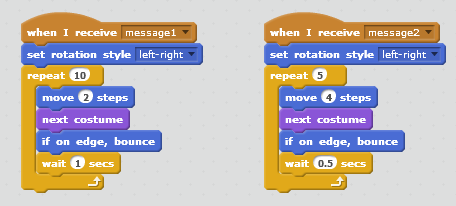
\includegraphics{img/CodeRepetition1.png}
  \caption{Two scripts repeating code}
  \label{fig:CodeRepetition1}
\end{figure}

\paragraph{}Estos scripts al ser analizados por el plug-in y traducidos a \textit{tokens} serían considerados iguales, ya que su código sería traducido al siguiente conjunto de bloques:
\begin{verbatim}
 'set rotation style %s'
 'repeat %s%s'
 'move %s steps'
 'next costume'
 'if on edge, bounce'
 'wait %s secs'
\end{verbatim}
\paragraph{} Así, la forma correcta de implementar este proyecto habría sido, tal como se muestra en la figura \ref{fig:CodeRepetition2}, definiendo un nuevo conjunto de bloques que recibe varios valores por parámetro y reutilizando el bloque creado en ambos programas, con las mejoras que esta solución implicaría en lo relativo al mantenimiento, actualización y depuración del código.

\begin{figure}
  \centering
    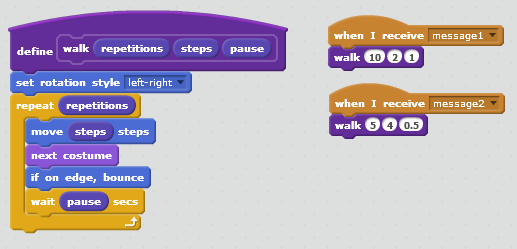
\includegraphics{img/CodeRepetition2.png}
  \caption{Defining own blocks to avoid code repetition}
  \label{fig:CodeRepetition2}
\end{figure}

\paragraph{}Para probar el funcionamiento de los plug-ins desarrollados y comprobar hasta qué punto estos comportamientos que habíamos detectado en nuestro trabajo se repiten también en los proyectos del repositorio de Scratch, procedimos a descargar 100 proyectos del mismo. Como la posibilidad de que los usuarios puedan definir sus propios bloques, con el uso del bloque \textit{def\_block}, solo se encuentra disponible desde el lanzamiento de Scratch 2.0, los proyectos descargados son todos posteriores a esta fecha.


\section{Findings}
\paragraph{}Los datos obtenidos tras analizar los 100 proyectos descargados confirman que las observaciones realizadas con nuestros estudiantes son también muy comunes en los proyectos de la comunidad. 
\paragraph{}En relación con la falta de costumbre de renombrar los personajes y no utilizar el nombre por defecto que asigna el entorno, el 79\% de los proyectos analizados contenían al menos un personaje sin renombrar del tipo \textit{SpriteX}.
\paragraph{}Como ejemplo para ilustrar los inconvenientes asociados a esta mala práctica se muestra en la imagen \ref{fig:SpriteNaming} un script que resulta difícilmente legible, ya que es necesario recorrer el área de personajes para localizar a qué personaje se refiere un bloque determinado, lo que dificulta la depuración del código ante eventuales problemas o mejoras e, incluso, ralentiza la propia programación por parte del estudiante, que debe memorizar o comprobar el número de objeto sobre el que quiere realizar una acción determinada.
\begin{figure}
  \centering
    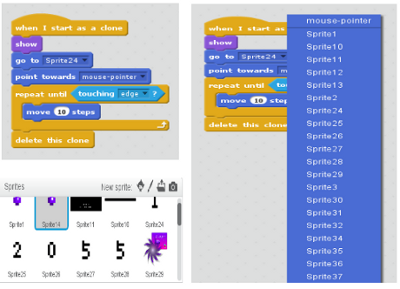
\includegraphics{img/SpriteNaming.png}
  \caption{Sprites with default names}
  \label{fig:SpriteNaming}
\end{figure}
\paragraph{}En cuanto a la repetición de código, el 62\% de los proyectos analizados contenían al menos un programa repetido. De hecho, tan solo el 17\% de los proyectos analizados hacían uso del bloque \textit{def\_block} para definirse un bloque propio y poder reutilizarlo en otras partes del proyecto.

\section{Conclussions}

\paragraph{} En lo relativo al nombrado de objetos, es curioso comprobar que los usuarios de Scratch sí nombran correctamente, es decir, de forma significativa, las variables que utilizan en sus proyectos. En nuestra opinión esto se debe a que cuando se crea una variable es obligatorio asignarle un nombre, ya que el entorno no las nombra por defecto. Sin embargo, al crear un nuevo personaje se le asinga el nombre \textit{SpriteX} de manera automática. Quizás una modificación del entorno para que obligue al usuario a nombrar a los nuevos objetos eliminaría esta mala práctica.
\paragraph{} En relación a la repetición de código y el poco uso que los usuarios de Scratch hacen de la definición de bloques propios (el equivalente a la creación de métodos o procedimientos en otros lenguajes), quizás trabajos como el realizado por Seiter y Foreman \cite{seiter2013modeling} en el que se pone de manifiesto que la capacidad de abstracción y la modularización son conceptos y habilidadades que parecen desarrollarse a partir de cierta edad, puedan explicar los bajos índices de uso de esta funcionalidad, ya que una parte importante de la comunidad Scratch está formada por niños menores de 10 años\footnote{http://scratch.mit.edu/statistics/\#age}. Futuros trabajos deberían seguir investigando en esta línea para continuar avanzando en la definición de un marco de trabajo apropiado para distintas edades y para comprobar si los usuarios que aprenden en línea y aquellos que lo hacen en un entorno reglado demuestran índices distintos de uso de esta funcionalidad. 

\newpage
\bibliography{scratch}
\bibliographystyle{unsrt}
\end{document}
